\documentclass[12pt]{article}

\usepackage{ucs}
\usepackage[utf8]{inputenc}
\usepackage{amssymb}
\usepackage[frenchb]{babel}
%\usepackage{fontenc}
%amazing maths packages
\DeclareUnicodeCharacter{00A0}{ }
\usepackage{array}
\usepackage{amsmath}
\usepackage{ragged2e}
\usepackage{tcolorbox}
\usepackage[a4paper,pdftex]{geometry}	% Use A4 paper margins
\usepackage{xcolor} % Required for specifying custom colors
\usepackage{fix-cm} % Allows increasing the font size of specific fonts beyond LaTeX default specifications
\usepackage{fancyhdr, graphicx}
\usepackage[normalem]{ulem}
\usepackage{fullpage}
\usepackage{graphicx}
\usepackage{tikz}

%matlab file inclusion

\usepackage{float}
\usepackage{listings}
\usepackage{color}
\definecolor{dkgreen}{rgb}{0,0.6,0}
\definecolor{gray}{rgb}{0.5,0.5,0.5}
\definecolor{mauve}{rgb}{0.58,0,0.82}

\lstset{frame=tb,
  language=Matlab,
  aboveskip=3mm,
  belowskip=3mm,
  showstringspaces=false,
  columns=flexible,
  basicstyle={\small\ttfamily},
  numbers=none,
  numberstyle=\tiny\color{gray},
  keywordstyle=\color{blue},
  commentstyle=\color{dkgreen},
  stringstyle=\color{mauve},
  breaklines=true,
  breakatwhitespace=true,
  tabsize=3
}

\newcommand*\tick{\item[\Checkmark]}
\newcommand*\fail{\item[\XSolidBrush]}
\newcommand*\bulet{\itemi[$\bullet$]}
\newcommand*\diamont{\item[$\diamond$]}

\setlength{\oddsidemargin}{0mm} % Adjust margins to center the colored title box
\setlength{\evensidemargin}{0mm} % Margins on even pages - only necessary if adding more content to this template

\newcommand{\HRule}[1]{\hfill \rule{0.2\linewidth}{#1}} % Horizontal rule at the bottom of the page, adjust width here

\definecolor{grey}{rgb}{0.9,0.9,0.9} % Color of the box surrounding the title - these values can be changed to give the box a different color	
%----------------------------------------------------------------------------------------
\title{Projet d'aide à la décision \\ Compte rendu client.}
\date{\today}
\author{Ségolène Minjard \and Salma El-Alaoui-Talibi \and Quentin Dupont \and Donovan Fournier \and Benjamin Legrand \and Zied Thabet \and Hexanôme H4304 \\ \\ Enseignants: Maryvonne \textsc{Miquel}
et Anne \textsc{Legait}  }

\begin{document}
\thispagestyle{empty} % Remove page numbering on this page

\renewcommand{\labelitemi}{$\bullet$}
%----------------------------------------------------------------------------------------
\colorbox{grey}{
	\parbox[t]{1.0\linewidth}{
		\centering \fontsize{40pt}{80pt}\selectfont % The first argument for fontsize is the font size of the text and the second is the line spacing - you may need to play with these for your particular title
		\vspace*{0.7cm} % Space between the start of the title and the top of the grey box
		
		\hfill Aide à la décision \\
		\hfill Compte rendu client\par
		
		\vspace*{0.7cm} % Space between the end of the title and the bottom of the grey box
	}
}

%----------------------------------------------------------------------------------------

\vfill % Space between the title box and author information

%----------------------------------------------------------------------------------------

{\centering \large 
\hfill Salma El Alaoui Talibi \\
\hfill Zied Thabet \\
\hfill Donovan Fournier \\
\hfill Ségolène Minjard \\
\hfill Benjamin Legrand \\
\hfill Quentin Dupont \\
\hfill \texttt{H 4304} \\

\HRule{1.5pt}} % Horizontal line, thickness changed here

%----------------------------------------------------------------------------------------

\clearpage % Whitespace to the end of the page

\vspace{25pt}
\setcounter{tocdepth}{2}
\tableofcontents % needs 2compilations
\pagebreak
%----------------------------------------------------------------------------------------
\section{Introduction}
\subsection{Contexte de l'étude}
Ce document est un compte rendu de l'étude menée par notre hexanôme H4304 pour le compte de la société FaBrique. Cette étude a pour but d'optimiser l'utilisation des ressources de l'entreprise en proposant le meilleur plan de production à mettre en place. \newline
En premier lieu, nous considèrerons indépendamment les objectifs métiers de chacun des cadres impliqués dans cette étude d'aide à la décision pour apporter une solution optimale à chacun.
En second lieu, nous proposerons au responsable d'entreprise une solution qui satisfait au mieux l'ensemble des points de vue.
Finalement, nous dégagerons parmi les 8 propositions de gestion de l'atelier, la solution optimale au vu des critères définis par les décideurs de l'entreprise.    
\subsection{Notations et conventions}
Nous expliquons dans ce paragraphe les notations qui seront adoptées dans la suite du document.
\begin{itemize}
\item Fonction objectif à optimiser pour le responsable.
\begin{align*} 
	\boldsymbol{Z_{poste\_responsable}}
\end{align*}
\item Vecteur où chaque composante $x_{i}$ représente la \underline{production hebdomadaire} du produit $i$. Les valeurs sont à $10^{-2}$ près.
\begin{align*} 
	\boldsymbol{X = 
   \left (
   \begin{array}{c}
      x_{A} \\
      x_{B} \\
      x_{C} \\
      x_{D} \\
      x_{E} \\
      x_{F} \\
   \end{array}
   \right )}
\end{align*}
\end{itemize}
Nous présenterons pour chaque responsable 3 résultats significatifs permettant d'analyser notre solution par rapport à l'objectif défini, il s'agit de :
\begin{itemize}
\item Vecteur $X^{*}$ (défini ci-dessus) où la fonction objectif atteint son optimum.
\begin{align*}
\boldsymbol{X^{*} = 
   \left (
   \begin{array}{c}
      x_{A} \\
      x_{B} \\
      x_{C} \\
      x_{D} \\
      x_{E} \\
      x_{F} \\
   \end{array}
   \right )}
 \end{align*}
 \item La valeur de la fonction objectif en cet optimum.
 \item Vecteur donnant la distance entre les contraintes et la solution optimale. Les valeurs sont arrondies à l'unité.
 \begin{align*} 
 \boldsymbol{A.X^{*}-b}
 \end{align*}
\end{itemize}
La matrice A est la matrice donnant les coefficients exprimant les contraintes et b le vecteur des seuils appliqués à chaque contrainte (cf section 2 - Prise en compte des contraintes globales). Ainsi, dans le vecteur plus la valeur est proche de 0 plus la contrainte correspondante a été satisfaite. 
\section{Prise en compte des contraintes globales}
\label{globconst}
Deux critères nous semblent limitants d'un point de vue de la production. En effet, les machines ne peuvent fonctionner qu'en présence des ouvriers et leurs horaires de travail sont limités. Il convient donc de limiter les temps d'utilisation de chacune d'elles.
En prenant en compte les durées de production respectives de chacun des produits sur les différentes machines, on introduit les 7 contraintes suivantes :
\begin{equation*}
\left\{
\begin{aligned}
    8x_{A} + 15x_{B} + 0x_{C} + 5x_{D} + 0x_{E} + 10x_{F} &\leq 4800
    \quad\\
      7x_{A} + 1x_{B} + 2x_{C} + 15x_{D} + 7x_{E} + 12x_{F} &\leq 4800 \\
      8x_{A} + 1x_{B} + 11x_{C} + 0x_{D} + 10x_{E} + 25x_{F} &\leq 4800 \\
      2x_{A} + 10x_{B} + 5x_{C} + 4x_{D} + 13x_{E} + 7x_{F} &\leq 4800 \\
      5x_{A} + 0x_{B} + 0x_{C} + 7x_{D} + 10x_{E} + 25x_{F} &\leq 4800 \\
      5x_{A} + 5x_{B} + 3x_{C} + 12x_{D} + 8x_{E} + 0x_{F} &\leq 4800 \\
      5x_{A} + 3x_{B} + 5x_{C} + 8x_{D} + 0x_{E} + 7x_{F} &\leq 4800 
\end{aligned}
\right.
\end{equation*}
De plus, la production est limitée par les matières premières. De fait, en appliquant les pondérations associées, on trouve :
\begin{equation*}
\left\{
\begin{aligned}
         1x_{A} + 2x_{B} + 1x_{C} + 5x_{D} + 0x_{E} + 2x_{F} &\leq 350 \quad\\
      2x_{A} + 2x_{B} + 1x_{C} + 2x_{D} + 2x_{E} + 2x_{F} &\leq 620 \\
      1x_{A} + 0x_{B} + 3x_{C} + 2x_{D} + 2x_{E} + 0x_{F} &\leq 485 \\
\end{aligned}
\right.
\end{equation*}
Il en découle les matrices A et b (définies à la section précédente) suivantes :
\begin{align*}
A =
 \begin{pmatrix}
  8	&15	&0 &5& 0 &10\\
7	&1	&2	&15	&7	&12\\
8	&1	&11	&0	&10	&25\\
2	&10	&5	&4	&13	&7\\
5	&0 &0 &7	&10   &25\\
5 &5 &3 &12 &8 &0\\
5 &3 &5 &8 &0 &7\\
1 &2 &1 &5 &0 &2\\
2 &2 &1 &2 &2 &2\\
1 &0 &3 &2 &2 &0
 \end{pmatrix}
  \quad b = 
   \left (
   \begin{aligned}
      4800 \\
      4800 \\
      4800 \\
      4800 \\
      4800 \\
      4800 \\
      4800\\
      350\\
      620\\
      485
   \end{aligned}
   \right ) 
 \end{align*}
 
Par ailleurs, nous devons ajouter des contraintes de domaines. En effet, la production ne peut pas être négative. Nous avons donc :
\(x_{A} \geq 0\), \(x_{B} \geq\), \(x_{C} \geq 0\), \(x_{D} \geq 0\), \(x_{E} \geq 0\), \(x_{F} \geq 0 \).
Des contraintes relatives aux différents cas d'analyses seront ajoutées aux précédentes par la suite.
\section{Analyse des objectifs de chacun des cadres}
Dans cette partie, nous mettons en œuvre des techniques de programmation linéaire mono-critère afin de proposer à chaque cadre la solution qui permet d'optimiser son objectif métier.
\subsection{Le comptable}
L'objectif du comptable est de maximiser le bénéfice de l'entreprise. Ce bénéfice est calculé en tenant compte des coûts de fonctionnement des machines et du coût d'achat des matières premières. Pour chaque produit le bénéfice unitaire (i.e. pour un produit vendu) sera donc donné par la formule suivante : 
\begin{equation*} 
pv - \sum_{i=1}^{3}(paMP_{i} * qteMP_{i}) - \frac{1}{60} \sum_{j=1}^{7}(tupM_{j} * chM_{j})  
\end{equation*}
\begin{description}
\item[$\boldsymbol{pv}$]\hfill \\Prix de vente du produit considéré fini.
\item[$\boldsymbol{paMP_{i}}$]\hfill \\ Le prix d'achat de la matière première de numéro i.
\item[$\boldsymbol{qteMP_{i}}$]\hfill \\ La quantité de matière première i, nécessaire pour la fabrication du produit considéré.
\item[$\boldsymbol{tupM_{j}}$]\hfill \\ Temps unitaire d'usinage du produit considéré sur la machine j.
\item[$\boldsymbol{chM_{j}}$]\hfill \\ Coût horaire de la machine j.
\end{description}
Il en ressort le problème de programmation linéaire mono-critère suivant:
\begin{tcolorbox}
Maximiser
\begin{align*}
Z_{comptable}= 5.67x_{A} +11.88x_{B} +12.27x_{C} +1.03x_{D} +31.65x_{E} +27.55x_{F}
\end{align*}
Sous les contraintes :
\begin{itemize}
\item contraintes globales (cf section 2 - Prise en compte des contraintes globales )
\end{itemize}
\end{tcolorbox}
On peut à partir des coefficients de la fonction objectif classer les produits selon le bénéfice unitaire qu'ils permettent de dégager. On obtient dans l'ordre décroissant de bénéfice unitaire : E, F, C, B, A, D.\\
La résolution mathématique de ce problème de programmation linéaire donne les résultats suivant :
\begin{align*} 
	\boldsymbol{X^{*}_{comptable} = 
   \left (
   \begin{aligned}
      x_{A} &= 0 \\
      x_{B} &= 20.41 \\
      x_{C} &= 0 \\
      x_{D} &= 0 \\
      x_{E} &= 242.50 \\
      x_{F} &= 94.18 
   \end{aligned}
   \right )}
\end{align*}
On constate que les produits les plus rentables (E puis F) sont beaucoup produits. Les produits
les moins rentables (A et D) ne sont pas du tout produits. Le produit C est légèrement plus rentable que le produit B mais B est préféré à C car il n'utilise pas la matière première 3 qui est beaucoup utilisée par E (présence d'une contrainte sur l'utilisation des matières premières).
\begin{align*}
\textbf{Bénéfice maximal = 10512 unités monétaires}
\end{align*}
Satisfaction des contraintes: 
\begin{align*} 
	\boldsymbol{A.X^{*}_{comptable} - b = 	
   \left(
   \begin{aligned}    
      -3552 \\
      -1952 \\
      0 \\
      -784 \\
      -20 \\
      -2758 \\
      -4080 \\
      -121 \\
      0 \\
      0\\
   \end{aligned}
   \right )}
\end{align*}
Les 7 premières lignes correspondent à l'utilisation des machines. On constate que les
machines 1 et 7 sont les moins utilisées. Ceci s'explique par le fait que ces machines ne sont
pas nécessaires pour produire E qui est le produit le plus réalisé. La machine 3 est utilisée au maximum car elle est très utilisée par les produits les plus réalisés (E et F). Les matières premières 2 et 3 sont consommées au maximum. En effet ce sont les matières premières nécessaires à la production de E. La production de E est ainsi poussée au maximum (jusqu'à épuisement des matières premières nécessaires).
\subsection{Le responsable d'atelier}
L'objectif du responsable d'atelier est de maximiser la quantité de produits fabriqués. 
Il en ressort le problème de programmation linéaire mono-critère suivant:
\begin{tcolorbox}
Maximiser
\begin{align*}
Z_{atelier}= x_{A} + x_{B} + x_{C} + x_{D} + x_{E} + x_{F}
\end{align*}
Sous les contraintes :
\begin{itemize}
\item contraintes globales (cf section 2 - Prise en compte des contraintes globales )
\end{itemize}
\end{tcolorbox}
La résolution mathématique de ce problème de programmation linéaire donne les résultats suivants:
\begin{align*} 
	\boldsymbol{X^{*}_{atelier} = 
   \left (
   \begin{aligned}
       x_{A} &= 0 \\
      x_{B} &= 56.73 \\
      x_{C} &= 38.69 \\
      x_{D} &= 0 \\
      x_{E} &= 184.46 \\
      x_{F} &= 98.92 
   \end{aligned}
   \right )
 }
\end{align*}
Nous remarquons que le modèle A n'est pas du tout produit car il mobilise toutes les machines ni le produit D car il mobilise en quantité toutes les matières premières. On produit en quantité les produits B, E et F car ils n'utilisent pas toutes les matières premières. On produit aussi du C car il n'utilise pas du tout 2 machines.
\begin{align*}
\textbf{Quantité maximale réalisée = 378.81 produits}
\end{align*}
La quantité est cohérente car celle-ci ne peut dépasser 620 (quantité maximale de matière
première 2, matière qui est toujours utilisée). La plupart des produits utilisent 2 unités de 
matière première 2 ce qui nous rapproche de 310. Les autres matières premières ont un maximum du même ordre de grandeur.\\
Satisfaction des contraintes :
\begin{align*} 
	\boldsymbol{A.X^{*}_{atelier} - b = 
   \left (
   \begin{aligned}
      -2960 \\
      -2188 \\
      0 \\
      -949 \\
      -482\\
      -2925 \\
      -3744 \\
      0 \\
      0 \\
      0\\
   \end{aligned}
   \right )}
\end{align*}
D'après les 3 dernières lignes, toutes les matières premières ont été utilisées au maximum, ce résultat est cohérent par rapport à l'objectif.
\subsection{Le responsable des stocks}
L'objectif du responsable des stocks est de minimiser le nombre de produits dans son stock. \\
Cette quantité est calculée en ajoutant le nombre de matières premières utilisées au nombre de produits usinés. Les coefficients de chaque produit sont donc calculés de la manière suivante : 
\begin{align*} C_{i} = 1 +  \sum_{j=1}^{3}(qteMP_{j}) 
\end{align*}
\begin{description}
\item[$\mathbf{C_{i}}$]\hfill\\Coefficient associé au produit i.
\item[$\mathbf{1}$]\hfill\\ Valeur correspondant au stockage du produit fini.
\item[$\mathbf{qteMP_{j}}$]\hfill\\La quantité de matière première j, nécessaire pour la fabrication du produit considéré.
\end{description}
Les contraintes globales, bien qu'elles prévoient des quantités fabriquées positives, ne suffisent pas pour assurer une activité minimale de l'entreprise. Et une tentative de résolution du problème du responsable de stock sans ajout de contraintes assurant l'activité minimale, aboutira à des quantités quasi nulle (de l'ordre de $ 10 ^{-16}$ ).\\
Nous avons donc ajouté la contrainte d'activité minimale suivante : le bénéfice de l'entreprise doit être supérieur à un certain pourcentage du bénéfice maximale.\\
Nous estimons donc que la contrainte suivante assure un certain fonctionnement de l'usine tout en restant raisonnable par rapport à l'objectif du responsable de stock : le bénéfice doit être supérieur ou égal à 50\% du bénéfice maximal. ($\frac{10512}{2} = 5256$ unités monétaires).\\
\\
Il en ressort le problème de programmation linéaire mono-critère suivant:
\begin{tcolorbox}
Minimiser
\begin{equation*}
 Z_{stocks}= 5x_{A} + 5x_{B} + 6x_{C} + 10x_{D} + 5x_{E} + 4x_{F}
\end{equation*}
Sous les contraintes :
\begin{itemize}
\item contraintes globales (cf section 2 - Prise en compte des contraintes globales )
\item $Z_{comptable}= 5.67x_{A} +11.88x_{B} +12.27x_{C} +1.03x_{D} +31.65x_{E} +27.55x_{F} \geq 5256$
\end{itemize}
\end{tcolorbox}
La résolution mathématique de ce problème de programmation linéaire donne les résultats suivants:
\begin{equation*}
\boldsymbol{X^{*}_{stocks} = 
   \left (
   \begin{aligned}
      x_{A} &= 0 \\
      x_{B} &= 0 \\
      x_{C} &= 0 \\
      x_{D} &= 0 \\
      x_{E} &= 13.74 \\
      x_{F} &= 175 
   \end{aligned}
   \right )
 } 
\end{equation*}
On remarque que le produit F est le plus fabriqué. De fait, il s'agit du produit qui utilise le moins de matières premières. Ensuite, les produits B et E consomment la même quantité de matières premières. Toutefois, les contraintes associées aux matières premières nous encouragent à préférer l'utilisation de la matière 3 par rapport à la matière 1 (Plus de disponibilité).
\begin{align*}
\textbf{Quantité minimale en stock = 768.70 éléments (Produits et matières premières)}
\end{align*}
Lors de la production, il faudra donc 769 places dans l'entrepôt pour stocker les marchandises (Produits finis ou matières premières). Toutes les places ne seront pas nécessairement occupées à tout instant (Notamment lors du processus de fabrication des produits).
\\
Satisfaction des contraintes : 
\begin{equation*}
\boldsymbol{A.X^{*}_{stocks} - b = 
   \left (
   \begin{aligned}
      -3050 \\
      -2604 \\
      -288 \\
      -3396\\
      -288 \\
      -4690 \\
      -3575 \\
      0\\
      -418 \\
      -458\\
      0\\
   \end{aligned}
   \right )
 } 
\end{equation*}
On remarque que la matière 1 est limitante car il est légitime de privilégier le produit F jusqu'à épuisement de la ressource 1.
On constate également que l'on pourrait utiliser plus de ressource 2 et 3 et les différentes machines. Néanmoins, le critère de bénéfice minimal étant atteint, la production est arrêtée malgré les disponibilités.

\subsubsection*{Analyse du résultat en fonction du bénéfice minimal}
Le graphe ci-dessous montre l'évolution du nombre de produits en stock en fonction de la contrainte du pourcentage de bénéfice minimal. 
\begin{figure}[H]
    \begin{center}
        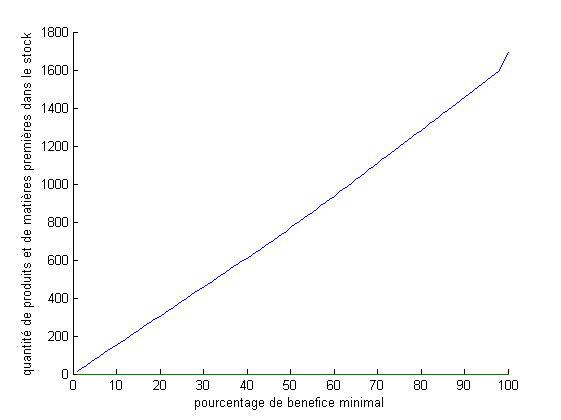
\includegraphics[scale=0.8]{plots_partie1/plot_stock.png}
        \caption{
            \label{fig} Évolution du stock en fonction de \%bénéfice minimal
        }
    \end{center}
\end{figure} 
La courbe montre une évolution linéaire de la quantité de produits stockés en fonction du pourcentage du bénéfice minimal.\\
\subsection{Le responsable commercial}
L'objectif du commercial est de conserver une certaine diversité dans sa gamme de produits tout en produisant le plus de produits. Concrètement, l'entreprise doit produire autant de produit de la gamme 1 (composée des produits A,B,C) que de la gamme 2 (composée des produits D,E,F).
On peut donc en déduire une contrainte d'égalité :
\begin{align*} 
(x_{a} + x_{b} + x_{c}) - (x_{d} + x_{e} + x_{f}) = 0
\end{align*}
De plus, il nous semble légitime de rajouter dans notre modèle le souhait de produire le plus de produits (comme dans le modèle du responsable atelier).
Il en ressort le problème de programmation linéaire mono-critère suivant :
\begin{tcolorbox}
Maximiser
\begin{equation*}
 Z_{commercial}(X)=x_{a} + x_{b} + x_{c} + x_{d} + x_{e} + x_{f}
\end{equation*}
Sous les contraintes :
\begin{itemize}
\item contraintes globales (cf section 2 - Prise en compte des contraintes globales )
\item $(x_{a} + x_{b} + x_{c}) - (x_{d} + x_{e} + x_{f}) = 0$
\end{itemize}
\end{tcolorbox}
La résolution mathématique de ce problème de programmation linéaire donne les résultats suivants :
\begin{align*}
\boldsymbol{X^{*}_{commercial} = 
   \left (
   \begin{aligned}
      x_{A} &= 142.12 \\
      x_{B} &= 0 \\
      x_{C} &= 44.42 \\
      x_{D} &= 0 \\
      x_{E} &= 104.81 \\
      x_{F} &= 81.73 \\
   \end{aligned}
   \right )
 } 
\end{align*}
On vérifie facilement que la contrainte inhérente au problème du commercial est respectée : le lot de produits \{A, B, C\} est usiné en même quantité que le lot de produits \{D, E, F\}. 
\begin{align*}
x_{A} + x_{B} + x_{C} = 142.12 + 0 + 44.42 = 186.54 \\
x_{D} + x_{E} + x_{F} = 0 + 104.81 + 81.73 = 186.54
\end{align*}
On remarque que les produits B et D sont totalement supprimés de la production. Cette particularité montre que le modèle B demande plus de ressources et/ou de temps de travail que ses modèles équivalents (A et C) et que d'un point de vue quantitatif, il est préférable de choisir ces derniers. 
\begin{align*}
\textbf{Quantité totale réalisée = 373.08 produits}
\end{align*}
On trouve une valeur cohérente par rapport à celle trouvée pour le chef d'atelier.\\
Satisfaction des contraintes : 
\begin{align*}
\boldsymbol{A.X^{*}_{commercial} - b = 
   \left (
   \begin{aligned}
      -2846 \\
      -2002 \\
      -83 \\
      -2359 \\
      -998 \\
      -3118 \\
      -3295 \\
      0 \\
      0 \\
      0
   \end{aligned}
   \right )
 } 
\end{align*}
Ces valeurs nous indiquent que les facteurs limitants de notre problème sont les ressources de production. Une augmentation de ces dernières permettrait de fabriquer plus de produits.
Dans ces conditions, la machine 7 est sous-exploitée tandis que la 3ème est presque en constante utilisation. Ces constatations sont explicables par l'importante production des modèles A, E et F. 
\subsection{Le responsable du personnel}
L'objectif du responsable du personnel est de minimiser l'usage des machines 3 et 5 (ces machines étant délicates).
Nous étudierons 3 cas de figures : 
\begin{itemize}
\item Minimiser le temps d'usage de la machine 3.
\item Minimiser le temps d'usage de la machine 5.
\item Minimiser la somme des temps d'usage des deux machines.
\end{itemize}
De même que pour le responsable des stocks, il faudra pour chacun de ces cas rajouter une contrainte assurant une  activité minimale de l'entreprise afin d'obtenir des quantités produites non nulles.\\ 

Nous avons donc retenu la même contrainte que pour le responsable des stocks, à savoir que le bénéfice de l'entreprise doit être supérieur à 50\% du bénéfice maximale ($\frac{10512}{2} = 5256$ unités monétaires).
\subsubsection{Limitation de l'usage de la machine 3}
Le problème de programmation linéaire monocritère posé ici est le suivant :
\begin{tcolorbox}
Minimiser
\begin{equation*}
 Z_{personnel/3}= 8x_{A} + x_{B} + 11x_{C} + 10x_{E} + 25x_{F}
\end{equation*}
Sous les contraintes :
\begin{itemize}
\item contraintes globales (cf section 2 - Prise en compte des contraintes globales )
\item $ Z_{comptable}= 5.67x_{A} +11.88x_{B} +12.27x_{C} +1.03x_{D} +31.65*x_{E} +27.55*x_{F} \geq 5256$
\end{itemize}
\end{tcolorbox}
La résolution mathématique de ce problème de programmation linéaire donne les résultats suivant :\\
\begin{equation*}
\boldsymbol{X^{*}_{personnel/3} = 
   \left (
   \begin{aligned}
      x_{A} &= 0 \\
      x_{B} &= 175.00 \\
      x_{C} &= 0 \\
      x_{D} &= 0 \\
      x_{E} &= 100.38 \\ 
      x_{F} &= 0 \\
   \end{aligned}
   \right )
 } 
\end{equation*}
\begin{align*}
\textbf{Usage minimal de la machine 3 = 1178.8 minutes/semaine}\\
\textbf{Usage de la machine 5 correspondant à ce plan = 1003.8 minutes/semaine}
\end{align*}
Satisfaction des contraintes : 
\begin{align*}
\boldsymbol{A.X^{*}_{personnel/3} - b = 
   \left (
   \begin{aligned}
      -2175 \\
      -3922 \\
      -3621 \\
      -1745 \\
      -3796 \\
      -3122 \\
      -4275 \\
      0 \\
      -69 \\
      -284\\
   \end{aligned}
   \right )
 } 
\end{align*}

\subsubsection{Limitation de l'usage de la machine 5}
Le problème de programmation linéaire monocritère posé ici est le suivant :
\begin{tcolorbox}
Minimiser
\begin{equation*}
 Z_{personnel/5}= 5x_{A} + 7x_{D} + 10x_{E} + 25x_{F}
\end{equation*}
Sous les contraintes :
\begin{itemize}
\item contraintes globales (cf section 2 - Prise en compte des contraintes globales )
\item $ Z_{comptable}= 5.67x_{A} +11.88x_{B} +12.27x_{C} +1.03x_{D} +31.65x_{E} +27.55x_{F} \geq 5256$
\end{itemize}
\end{tcolorbox}
La résolution mathématique de ce problème de programmation linéaire donne les résultats suivant :\\
\begin{equation*}
\boldsymbol{X^{*}_{personnel/5} = 
   \left (
   \begin{aligned}
      x_{A} &= 0 \\
      x_{B} &= 120.34 \\
      x_{C} &= 109.32 \\
      x_{D} &= 0 \\
      x_{E} &= 78.52 \\ 
      x_{F} &= 0 \\
   \end{aligned}
   \right )
 } 
\end{equation*}
\begin{align*}
\textbf{Usage minimal de la machine 5 = 785 minutes/semaine} \\
\textbf{Usage de la machine 3 correspondant à ce plan = 2104 minutes/semaine}
\end{align*}


Satisfaction des contraintes : 
\begin{align*}
\boldsymbol{A.X^{*}_{personnel/5} - b = 
   \left (
   \begin{aligned}
      -2995 \\
      -3911 \\
      -2692 \\
      -2029 \\
      -4015 \\
      -3242 \\
      -4892 \\
      0 \\
      -113 \\
      0\\
   \end{aligned}
   \right )
 } 
\end{align*}
\subsubsection{Limitation de l'usage des machines 3 et 5} 
On calcule donc les temps passés sur les machines pour chaque produit, d'où la formule suivante permettant de calculer les coefficients de la fonction : 
\begin{align*} 
 C_{i} = \sum_{j\in\lbrace3;5\rbrace}tupM_{j} 
 \end{align*} 
\begin{description}
\item[$\boldsymbol{C_{i}}$] \hfill\\Coefficient associé au produit i.
\item[$\boldsymbol{tupM_{j}}$]\hfill\\ Temps unitaire d'usinage du produit considéré sur la machine j.
\end{description}
De même que pour le responsable des stocks, il faudra rajouter ici une contrainte assurant une  activité minimale de l'entreprise afin d'obtenir des quantités produites non nulles. Nous avons retenu la même contrainte, à savoir que le bénéfice de l'entreprise doit être supérieur à 50\% du bénéfice maximale.
Il en ressort le problème de programmation linéaire mono-critère suivant :
\begin{tcolorbox}
Minimiser
\begin{equation*}
 Z_{personnel}= 13x_{A} + x_{B} + 11x_{C} + 7x_{D} + 20x_{E} + 50x_{F}
\end{equation*}
Sous les contraintes :
\begin{itemize}
\item contraintes globales (cf section 2 - Prise en compte des contraintes globales )
\item $ Z_{comptable}= 5.67x_{A} +11.88x_{B} +12.27x_{C} +1.03x_{D} +31.65*x_{E} +27.55*x_{F} \geq 5256$
\end{itemize}
\end{tcolorbox}
La résolution mathématique de ce problème de programmation linéaire donne les résultats suivant :\\
\begin{equation*}
\boldsymbol{X^{*}_{personnel} = 
   \left (
   \begin{aligned}
      x_{A} &= 0 \\
      x_{B} &= 175.00 \\
      x_{C} &= 0 \\
      x_{D} &= 0 \\
      x_{E} &= 100.38 \\ 
      x_{F} &= 0 \\
   \end{aligned}
   \right )
 } 
\end{equation*}
On constate qu'il est préférable de fabriquer les produits B et E. En effet, le produit B ne demande qu'une minute de temps d'utilisation cumulé sur les 2 machines, il semble donc correspondre au mieux aux critères. La production seule de ce produits ne permettant pas d'atteindre le seuil de rentabilité défini précédemment, il est nécessaire de produire une autre gamme. Malgré son fort taux d'utilisation, le produit E a été choisi pour compléter la production. L'analyse de la satisfaction des contraintes nous permet de comprendre cette préférence.
\begin{align*}
\textbf{Usage minimal des machines = 2182.7 minutes/semaine}\\
\Longleftrightarrow
\textbf{Usage de la machine 3 = 1178.8 minutes/semaine}\\
\textbf{Usage de la machine 5 = 1003.8 minutes/semaine}
\end{align*}
Satisfaction des contraintes : 
\begin{align*}
\boldsymbol{A.X^{*}_{personnel} - b = 
   \left (
   \begin{aligned}
      -2175 \\
      -3922 \\
      -3612 \\
      -1745 \\
      -3792 \\
      -3122 \\
      -4275 \\
      0 \\
      -69 \\
      -284\\
   \end{aligned}
   \right )
 } 
\end{align*}
Bien que le produit B ait été préférable, sa production est limitée par la quantité de matière première 1 (Contrainte nulle). Il a donc fallu compléter la production avec un produit n'utilisant pas cette matière, seul le produit E correspond à ce critère d'où sa production en second choix.
Comme pour le cas du responsable des Stocks, il est encore possible d'augmenter la production (MP 2 et 3 ne sont pas écoulées). Néanmoins, le plan de production donné ici respecte la contrainte de minimum de chiffre d'affaire donnée en début de partie.

\subsubsection*{Analyse du résultat en fonction du bénéfice minimal}
Les courbes ci-dessous tracent l'évolution du temps d'usage des machines 3 et 5 dans le cas de l'optimisation sur la somme des temps d'usage. 
\begin{figure}[H]
    \begin{center}
        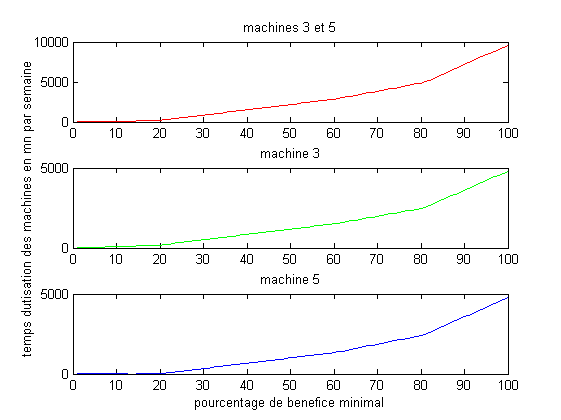
\includegraphics[scale=0.8]{plots_partie1/plot_personnel.png}
        \caption{
            \label{fig} Évolution des temps des machines 3 et 5 en fonction du\%bénéfice minimal
        }
    \end{center}
\end{figure} 
Les courbes montrent que les contraintes de bénéfices minimal acceptables sont dans la plage [25\% - 80\%] du bénéfice max. Au delà de 80\% l'utilisation des machines 3 et 5 croit de façon plus rapide. Des contraintes supérieurs à 80\% du bénéfice maximum sont donc à écarter.  \\

\subsubsection{Conclusion}
Au vu des différents résultats obtenus pour les 3 cas, nous concluons que la solution à retenir est celle qui minimise la machine 3 ou la somme des temps des deux machines (ces deux solutions étant équivalentes).  La solution qui minimise uniquement l'usage de la machine 5 est à rejeter car elle entraine une utilisation excessive de la machine 3. 
\section{Point de vue du Responsable d'entreprise}
Nous avons défini la matrice de gain suivante:
\begin{align*}
Matrice de Gain =
 \begin{pmatrix}
    10512    &357   &1691    &316   &9580   &4800   &4780\\
    9712     &379   &1834    &188   &9118   &4800   &4318\\
    5256    &189    &769    &189     &9025   &4512   &4512\\
    6920    &373   &1828    &0       &8519    &4717   &3802\\
    5256    &275   &1377    &75     &2183    &1179   &1004\\
    5256    &275   &1377   &75     &2183    &1179   &1004\\
    5256    &308   &1650    &151   &2893    &2108    &785
 \end{pmatrix}
\end{align*}\\

Cette matrice représente les objectifs de chacun des cadres (en colonnes) et des solutions optimales calculées en prenant les objectif séparément (en lignes). Les colonnes indiquent (de gauche à droite),le bénéfice, la production totale, le nombre de produits et matières premières en stock, l'écart entre la production des 2 gammes de produits, le temps d'utilisation total des machines 3 et 5, le temps d'utilisation de la machine 3 et enfin le temps d'utilisation de la machine 5.

A partir de cette matrice, nous avons élaborée une solution de compromis en définissant des seuils de satisfaction minimale pour chacun des objectifs. Nous avons donc reformulé le problème avec comme fonction objectif à maximiser le bénéfice(qui nous semble être l'intérêt premier du responsable d'entreprise), avec des contraintes supplémentaires correspondant à la satisfaction des objectifs des autres cadres. 

Notre \textbf{point de mire} correspond à la diagonale de la matrice de gain, c'est à dire aux valeurs optimales pour chaque cadre:
\begin{itemize}
\item \textbf{10512} d'unités monétaires
\item  \textbf{379} de produits réalisés
\item \textbf{769} de produits et matières premières en stock
\item \textbf{0} de différence de produits entre les 2 catégories (A, B, C) et (D, E, F).
\item \textbf{2183} de minutes/semaine d'usages pour les machines 3 et 5. Cela correspond à \textbf{1179} minutes/semaine pour la machine 3 et à \textbf{1004} minutes/semaine pour la machine 5.
\end{itemize}
C'est de ce point que nous allons essayer de nous rapprocher, en essayant de trouver un compromis qui satisfera les différents responsables.
\\ \\
Nous obtenons ainsi le problème de programmation linéaire suivant :
\begin{tcolorbox}
Maximiser
\begin{equation*}
 Z_{comptable}= 5.67x_{A} +11.88x_{B} +12.27x_{C} +1.03x_{D} +31.65x_{E} +27.55x_{F}
\end{equation*}
Sous les contraintes :
\begin{itemize}
\item contraintes globales (cf section 2 - Prise en compte des contraintes globales )
\item nouvelles contraintes déduites des fonctions objectifs des autres cadres:\\
\end{itemize}
\begin{equation*}
\left\{
\begin{aligned}
   Z_{atelier}= x_{A} + x_{B} + x_{C} + x_{D} + x_{E} + x_{F} &\geq seuil_{atelier}
    \\
   Z_{stocks}= 5x_{A} + 5x_{B} + 6x_{C} + 10x_{D} + 5x_{E} + 4x_{F}
   &\leq seuil_{stock}
   \\
   Z_{commercial}(X)=x_{a} + x_{b} + x_{c} + x_{d} + x_{e} + x_{f} &\geq seuil_{commercial}
   \\
   Z_{personnel}= 13x_{A} + x_{B} + 11x_{C} + 7x_{D} + 20x_{E} + 50x_{F}&\leq seuil_{personnel}
\end{aligned}
\right.
\\
\newline
\end{equation*}
\end{tcolorbox}
Il s'agit maintenant de déterminer les seuils de satisfaction ci-dessus. Nous les fixons tout d'abord aux valeurs de la médiane de chaque colonne de la matrice de gain. Nous essayons ensuite de dégrader les contraintes sur plusieurs itérations pour essayer de nous rapprocher au plus du point de mire. La stratégie du responsable d'entreprise étant de maximiser le bénéfice, nous considérons qu'il est cohérent d'accorder plus d'importance aux fonctions atelier et commercial, et nous appliquons des contraintes moins sévères pour les fonctions stock et personnel.

A chaque itérations, nous estimons le rapprochement entre les valeurs obtenues pour chaque responsable et le point de mire en fonction du modèle suivant:
 
Nous définissons le \textbf{pourcentage d'erreur} comme:
	\begin{equation*}
		\boldsymbol{\%erreur=|(valeur_{responsable}-valeur Optimale_{responsable}|}
	\end{equation*}
et la \textbf{réponse aux exigences} des cadres comme:
	\begin{equation*}
		\boldsymbol{max(0, 1-\%erreur)}
	\end{equation*}
Le maximum empêche l’obtention de valeurs négatives qui n’auraient aucun sens métier.
Pour le responsable commercial, la formule est différente car on cherche à réduire l’écart entre les deux catégories de produits. 
Le pourcentage d’erreur est donc défini comme étant:
\begin{equation*}
		\boldsymbol{\%erreur=\frac{(A+B+C)-(D+E+F)}{A+B+C+D+E+F}}
	\end{equation*}
A, B, C, D, E, F représentant la quantité du produit correspondant.On remet ainsi l'écart à l'échelle de la production.

\noindent Ce modèle traduit le fait suivant: nous estimons qu'obtenir une valeur deux fois plus grande que la valeur optimale pour un objectif à minimiser (ou deux fois plus petite si l'objectif est à maximiser) est trop loin de nos exigences. Dans ce cas l'erreur est supérieure à 1 et la réponse aux exigences est de 0.

Les seuils que nous obtenons sont:
\begin{equation*}
\left\{
\begin{aligned}
   Z_{atelier}= x_{A} + x_{B} + x_{C} + x_{D} + x_{E} + x_{F} &\geq290 
    \\
   Z_{stocks}= 5x_{A} + 5x_{B} + 6x_{C} + 10x_{D} + 5x_{E} + 4x_{F}
   &\leq1450 
   \\
   Z_{commercial}(X)=x_{a} + x_{b} + x_{c} + x_{d} + x_{e} + x_{f} &\geq 10
   \\
   Z_{personnel}= 13x_{A} + x_{B} + 11x_{C} + 7x_{D} + 20x_{E} + 50x_{F}&\leq 4000
\end{aligned}
\right.
\\
\\
\end{equation*}
Cela donne le plan de production suivant:
\begin{itemize}
\item \textbf{7305} d'unités monétaires
\item  \textbf{2900} de produits réalisés
\item \textbf{1450} de produits et matières premières en stock
\item \textbf{100} de différence de produits entre les 2 catégories (A, B, C) et (D, E, F).
\item \textbf{4000} de minutes/semaine d'usages pour les machines 3 et 5. Cela correspond à \textbf{2047} minutes/semaine pour la machine 3 et à 1952 minutes/semaine pour la machine 5.
\end{itemize}
Ce plan correspond à un niveau de réponse aux exigences des différents cadres suivant:
\begin{figure}[H]
    \begin{center}
        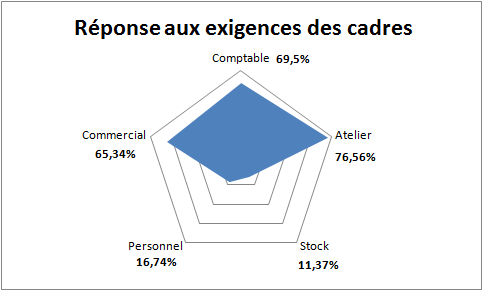
\includegraphics[scale=0.8]{plots_partie2/plot_radar.png}
        \caption{
            \label{fig} Réponse aux exigences des cadres
        }
    \end{center}
\end{figure}
\subsection*{Conclusion}
La solution qu'on propose est satisfaisante car privilégie le bénéfice et la productivité tout en conservant des valeurs acceptables pour les objectifs des autres cadres.

\noindent Ainsi, dans la partie suivante, nous accorderons d'avantage d'importance aux critères de bénéfice et de productivité.

\section{Sélection du meilleur plan de production}
Suite aux études précédentes et aux différentes discussions, nous avons retenu 8 propositions de gestion d'atelier (notées de \textbf{\emph{a}} à \textbf{\emph{h}}).\\
Les décideurs de l'entreprise se sont entendus sur 4 critères à considérer pour décider du meilleur plan de production : le bénéfice, la gestion du stock, l'équilibre commercial (proposer une diversité de produits) et le taux d'utilisation de certaines machines délicates.\\
Pour résoudre ce problème et trouver la meilleure solution possible, nous avons utilisé la méthode \emph{Electre I}.\\
Dans un premier temps, nous avons déterminé grâce à la matrice de jugements les dominances fortes sur les critères précédents. Ainsi, nous avons déterminé que :
\begin{itemize}
\item \textbf{\emph{b}} et \textbf{\emph{h}} dominent \textbf{\emph{c}}
\item \textbf{\emph{e}} domine \textbf{\emph{g}}
\item \textbf{\emph{h}} domine \textbf{\emph{f}}
\end{itemize}
Nous ne prenons donc plus en compte les propositions \textbf{\emph{c}}, \textbf{\emph{g}} et \textbf{\emph{f}} .\\
Nous avons par la suite déroulé la méthode Electre I dans deux cas différents. 
\begin{itemize}
\item Sans accorder de poids aux différents critères.
\item En pondérant chacun des critères.
\end{itemize}
\subsection{Analyse sans pondération des critères}
Nous obtenons les matrices de concordance (C) et discordance (D) suivante : \\
\begin{minipage}{0.45\textwidth}
C = $\frac{1}{4}$*\bordermatrix{
				  ~ & a & b & d & e & h \cr
                  a & - & 3 & 3 & 3 & 3 \cr
                  b & 1 & - & 2 & 3 & 2 \cr
                  d & 2 & 2 & - & 2 & 3 \cr
                  e & 1 & 3 & 2 & - & 2 \cr
                  h & 2 & 2 & 3 & 2 & - \cr}
\end{minipage}
~
\begin{minipage}{0.45\textwidth}
D = $\frac{1}{10}$*\bordermatrix{
				  ~ & a & b & d & e & h \cr
                  a & - & 4 & 2 & 4 & 2 \cr
                  b & 2 & - & 3 & 6 & 1 \cr
                  d & 3 & 4 & - & 5 & 2 \cr
                  e & 2 & 6 & 3 & - & 4 \cr
                  h & 3 & 2 & 2 & 5 & - \cr}
\end{minipage}\\[0.5cm]
En nous basant sur ces matrices et en fixant différents seuils de concordance/discordance, nous traçons les graphes de surclassement suivants :\\
\vspace{10pt}
\fbox{\begin{minipage}{0.3\textwidth}
$C_1=\frac{3}{4}$; $C_2=\frac{2}{10}$ \\
\begin{tikzpicture}[->,auto,node distance=1.5cm,thick,
   mauvaise action/.style={font=\sffamily\Large\bfseries},
   bonne action/.style={circle,draw,font=\sffamily\Large\bfseries}]

  \node[bonne action](a) {a};
  \node[bonne action](b) [below right of=a] {b};
  \node[mauvaise action](d) [below of=b] {d};
  \node[mauvaise action](h) [below left of=a] {h};
  \node[bonne action](e) [below of=h] {e};

  \foreach \from/\to in {a/d,a/h,d/h, h/d} \draw (\from) -- (\to);
\end{tikzpicture}\\
\centering
ensemble des meilleures actions potentielles = \{a,b,e\}
\end{minipage}}
\fbox{\begin{minipage}{0.3\textwidth}
$C_1=\frac{2}{4}$; $C_2=\frac{2}{10}$ \\
\begin{tikzpicture}[->,auto,node distance=1.5cm,thick,
   mauvaise action/.style={font=\sffamily\Large\bfseries},
   bonne action/.style={circle,draw,font=\sffamily\Large\bfseries}]

  \node[bonne action](a) {a};
  \node[mauvaise action](b) [below right of=a] {b};
  \node[mauvaise action](d) [below of=b] {d};
  \node[mauvaise action](h) [below left of=a] {h};
  \node[bonne action](e) [below of=h] {e};

  \foreach \from/\to in {a/d,a/h,b/h,d/h,h/b,h/d} \draw (\from) -- (\to);
\end{tikzpicture}\\
\centering
ensemble des meilleures actions potentielles = \newline\{a,e\}
\end{minipage}}
\fbox{\begin{minipage}{0.3\textwidth}
$C_1=\frac{3}{4}$; $C_2=\frac{4}{10}$ \\
\begin{tikzpicture}[->,auto,node distance=1.5cm,thick,
   mauvaise action/.style={font=\sffamily\Large\bfseries},
   bonne action/.style={circle,draw,font=\sffamily\Large\bfseries}]

  \node[bonne action](a) {a};
  \node[mauvaise action](b) [below right of=a] {b};
  \node[mauvaise action](d) [below of=b] {d};
  \node[mauvaise action](h) [below left of=a] {h};
  \node[mauvaise action](e) [below of=h] {e};

  \foreach \from/\to in {a/b,a/d,a/e,a/h,d/h, h/d} \draw (\from) -- (\to);
\end{tikzpicture}\\
\centering
ensemble des meilleures actions potentielles = \newline\{a\}
\end{minipage}}
\\
En analysant les différents graphes, on peut déduire que le plan de production A serait le plan répondant le mieux aux critères malgré un léger effet de rattrapage (Augmentation du coefficient C$_{2}$ requise).

~
\subsection{Analyse avec pondération des critères} 
Nous avons ensuite attribué un poids à chacun de ces critères en jugeant de leur importance relative et au vu des résultats de la partie 2. Nous privilégions principalement le bénéfice (raison d'être de l'entreprise) auquel nous affectons un poids fort égal à 5. Nous avons ensuite décider d'affecter une pondération moyenne égale à 3 au critère 3 garantissant une production de produits diversifiée. Quant aux critères 2 et 4, nous les considérons comme les moins importants (poids faible égal à 2), vu que les opérateurs peuvent être formés à l'utilisation des machines et que le maintien d'un stock minimal n'est pas d'une importance primordiale.\\
Pour notre analyse, nous avons réévalué les notes de chaque critère afin de correspondre à une échelle plus adaptée. Nous obtenons donc une nouvelle matrice de jugements, ainsi que de nouvelles matrices de concordance et de discordance, sans les propositions dominées \textbf{\emph{c}}, \textbf{\emph{g}} et \textbf{\emph{f}} :
\begin{center}
\newcolumntype{M}{>{\centering\arraybackslash} m{1.5cm} }
\newcolumntype{L}{>{\centering\arraybackslash} m{1.75cm} }
\renewcommand{\arraystretch}{1.2}
\begin{tabular}{|L|M|M|M|M|}
\hline 
Critère & g1 & g2 & g3 & g4 \\\hline  
Coefficient & 5 & 2 & 3 & 2 \\ \hline 
Echelle & 0 $ \Rightarrow $ 10 & 3 $ \Rightarrow $ 7 & 2 $ \Rightarrow $ 8 & 3 $ \Rightarrow $ 7 \\ \hline 
a & 6 & 5 & 5 & 5 \\ \hline 
b & 5 & 4.6 & 7.4 & 4.2 \\ \hline 
c & 3 & 4.6 & 6.2 & 4.2 \\ \hline 
d & 3 & 5.8 & 5 & 4.6 \\ \hline 
e & 5 & 4.6 & 3.8 & 6.6 \\ \hline 
f & 2 & 5 & 6.2 & 4.2 \\ \hline 
g & 5 & 4.6 & 3.2 & 6.6 \\ \hline 
h & 3 & 5 & 6.2 & 4.6 \\ 
\hline 
\end{tabular} 
\end{center}
\begin{minipage}{0.45\textwidth}
C = $\frac{1}{12}$*\bordermatrix{~ & a & b & d & e & h \cr
                  a & - & 9 & 10 & 10 & 9 \cr
                  b & 3 & - & 8 & 10 & 8 \cr
                  d & 5 & 4 & - & 5 & 9 \cr
                  e & 2 & 9 & 7 & - & 7 \cr
                  h & 5 & 4 & 10 & 5 & - \cr}
\end{minipage}
~
\begin{minipage}{0.45\textwidth}
D = $\frac{1}{10}$*\bordermatrix{~ & a & b & d & e & h \cr
                  a & - & 2.4 & 0.8 & 1.6 & 1.2 \cr
                  b & 1.0 & - & 1.2 & 2.4 & 0.4 \cr
                  d & 3.0 & 2.4 & - & 2.0 & 1.2 \cr
                  e & 1.2 & 3.6 & 1.2 & - & 2.4 \cr
                  h & 3.0 & 2.0 & 0.8 & 2.0 & - \cr}
\end{minipage}\\[0.5cm]
Nous avons appliqué 4 seuillages en modifiant seuil de concordance et discordance afin de déterminer le meilleur plan de production. Voici les graphes de surclassement qui en résultent : \\
\vspace{10pt}
\fbox{\begin{minipage}{0.2\textwidth}
Strict :
$C_1=\frac{10}{12}$; $D_1=\frac{1.5}{10}$ \\
\begin{tikzpicture}[->,auto,node distance=1.5cm,thick,
   mauvaise action/.style={font=\sffamily\Large\bfseries},
   bonne action/.style={circle,draw,font=\sffamily\Large\bfseries}]

  \node[bonne action] (a) {a};
  \node[bonne action](b) [below right of=a] {b};
  \node[mauvaise action] (d) [below of=b] {d};
  \node[bonne action] (h) [below left of=a] {h};
  \node[bonne action] (e) [below of=h] {e};

  \foreach \from/\to in {a/d,h/d} \draw (\from) -- (\to);
\end{tikzpicture}\\
\centering
meilleures actions potentielles = \{a,b,e,h\}
\end{minipage}}
~
\vspace{10pt}
\fbox{\begin{minipage}{0.2\textwidth}
Moyen strict:
$C_2=\frac{10}{12}$; $D_2=\frac{2}{10}$ \\
\begin{tikzpicture}[->,auto,node distance=1.5cm,thick,
   mauvaise action/.style={font=\sffamily\Large\bfseries},
   bonne action/.style={circle,draw,font=\sffamily\Large\bfseries}]

  \node[bonne action] (a) {a};
  \node[bonne action](b) [below right of=a] {b};
  \node[mauvaise action] (d) [below of=b] {d};
  \node[bonne action] (h) [below left of=a] {h};
  \node[mauvaise action] (e) [below of=h] {e};

  \foreach \from/\to in {a/d,a/e,h/d} \draw (\from) -- (\to);
\end{tikzpicture}\\
\centering
meilleures actions potentielles = \{a,b,h\}
\end{minipage}}
~
\vspace{10pt}
\fbox{\begin{minipage}{0.2\textwidth}
Moyen : 
$C_2=\frac{8}{12}$; $D_2=\frac{2}{10}$ \\
\begin{tikzpicture}[->,auto,node distance=1.5cm,thick,
   mauvaise action/.style={font=\sffamily\Large\bfseries},
   bonne action/.style={circle,draw,font=\sffamily\Large\bfseries}]

  \node[bonne action] (a) {a};
  \node[bonne action](b) [below right of=a] {b};
  \node[mauvaise action] (d) [below of=b] {d};
  \node[mauvaise action] (h) [below left of=a] {h};
  \node[mauvaise action] (e) [below of=h] {e};

  \foreach \from/\to in {a/d,a/e,h/d,a/h,d/h,b/d,b/h} \draw (\from) -- (\to);
\end{tikzpicture}\\
\centering
meilleures actions potentielles = \{a,b\}
\end{minipage}}
~
\vspace{10pt}
\fbox{\begin{minipage}{0.2\textwidth}
Lâche : 
$C_2=\frac{8}{12}$; $D_2=\frac{2.5}{10}$ \\
\begin{tikzpicture}[->,auto,node distance=1.5cm,thick,
   mauvaise action/.style={font=\sffamily\Large\bfseries},
   bonne action/.style={circle,draw,font=\sffamily\Large\bfseries}]

  \node[bonne action] (a) {a};
  \node[mauvaise action](b) [below right of=a] {b};
  \node[mauvaise action] (d) [below of=b] {d};
  \node[mauvaise action] (h) [below left of=a] {h};
  \node[mauvaise action] (e) [below of=h] {e};

  \foreach \from/\to in {a/d,a/b,a/e,a/h,b/d,b/e,b/h,d/h,h/d} \draw (\from) -- (\to);
\end{tikzpicture}\\
\centering
meilleures actions potentielles = \{a\}
\end{minipage}}
\\Avec le seuillage strict, nous ne pouvons pas déterminer de meilleurs solutions car nous ne pouvons comparer les comportements des plans de production \textbf{\emph{a}}, \textbf{\emph{b}} et \textbf{\emph{e}}. En augmentant les seuils de concordance et discordance, nous voyons se dégager des meilleurs actions potentielles. En relâchant les seuils, nous arrivons à comparer des plans de productions ayant des comportements différents. En effet, avec le seuillage moyen, les solutions \textbf{\emph{a}} et \textbf{\emph{b}} ressortent. Tandis que le plan \textbf{\emph{a}} est stable pour les quatre critères, le plan \textbf{\emph{b}} rattrape ses résultats faibles (\textbf{\emph{g2}} et \textbf{\emph{g4}}) avec le critère \textbf{\emph{g3}}.
Finalement, nous pouvons conclure que le plan \textbf{\emph{a}} est la meilleure solution. Cela s'explique grâce à ses résultats stables et son bon résultat au seul critère de poids fort (\textbf{\emph{g1}}) où il obtient 6 sur 10, la meilleure note sur ce critère.
\newpage
\section{Annexe}
\subsection{Description du problème}
\lstinputlisting{../Probleme.m}
\subsection{Description des différents objectifs des cadres}
\subsubsection{Atelier}
\lstinputlisting{../Atelier.m}
\subsubsection{Commercial}
\lstinputlisting{../Commercial.m}
\subsubsection{Comptable}
\lstinputlisting{../Comptable.m}
\subsubsection{Personnel}
\lstinputlisting{../Personnel.m}
\subsubsection{Stock}
\lstinputlisting{../Stock.m}
\subsection{Point de vue du Responsable d'entreprise}
\subsubsection{Matrice de gain}
\lstinputlisting{../MatriceGain.m}
\subsubsection{Taux de satisfaction}
\lstinputlisting{../Satisfaction.m}
\subsection{Selection du meilleur plan de production}
\subsubsection{Changement d'échelle}
\lstinputlisting{../changement_echelle.m}
\subsubsection{Calcul de la concordance}
\lstinputlisting{../concordance.m}
\subsubsection{Calcul de la discordance}
\lstinputlisting{../discordance.m}
\subsubsection{Seuillage Electre}
\lstinputlisting{../seuillage_electre.m}
\end{document}
